\subsection{The transiting planet model \label{transit_model}}
To actually model the starspot features within the transit portions of the light curve, a reasonable understanding of the visibility profile of a transit for any given system is required. The visibility of the transits is determined by the portion of the star that the planet occludes during transit and limb darkening effects. As discussed earlier, the planet will only transit along the boxes contained within the latitudes at $cos^{-1}(R_p \pm b$. 
 
The first step in determining the visibility occluded by a planet at a given time step involves geometry which will be extended to the ten cases contained in Table~\ref{cases}. The simplifying approximation that each of the boxes is a cartesian rectangle when it is projected onto the surface of the star is made. The midpoints of the edges of the cartesian rectangle are the same as the midpoints of the projected box edges. The top and bottom of the cartesian rectangles are the same as the projected rectangles. Although this is not entirely accurate, it is a good approximation because when a cartesian rectangle overestimates a portion of the projected box, it must also underestimate a similar but not necessarily equal portion of the box. Near the limbs, the curvature of the projected boxes as compared to the cartesian rectangles becomes more extreme, however the cartesian rectangles become smaller so that although the relative area misappropriated may be larger, the absolute error is smaller.

The simplest case in which the planet is entirely contained within a box is:
\begin{equation}
	A_{occluded} = \pi r_p^2
\end{equation}

The planet can also be partially contained in a box in many ways, shown in Table~\ref{cases}. The sliver of the planet that is not within the box will be calculated and then extended to take care of all of the various cases. To do this, the area of a sector of a circle is found and then the triangle that is formed within it is subtracted. The sector is the combination of the light blue and yellow regions in Figure~\ref{eclipse}.
\begin{figure}[h]
	\centering
	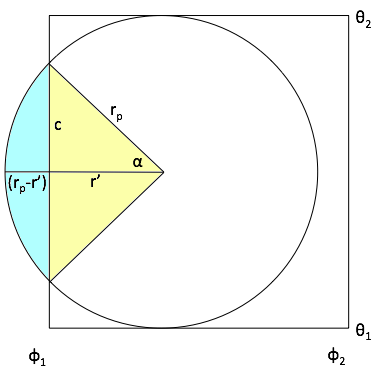
\includegraphics[width=.5\textwidth]{images/figure.png}
	\caption{Geometry of eclipse path visibility.}
	\label{eclipse}
\end{figure}

\begin{equation}
	A_{sector} = \frac{r_p \alpha^2}{2}
\end{equation}

where:

\begin{equation}
	\alpha = 2 \cos^{-1}\left(\frac{r^{\prime}}{r_p}\right)
\end{equation}

The area of the triangle is $cr^{\prime}$. $c$ is one half the length of the chord in the figure. $c$ can be found with the Pythagorean theorem. Knowing this, the area of the triangle becomes: 

\begin{equation}
	A_{triangle} = r^{\prime}\sqrt{r_p^2 - {r^{\prime}}^2}
\end{equation}

Finally, the area of the segment that indicates the part of the planet just over the border of the box is:

\begin{equation}
	A_{seg} = r_p^2 \cos^{-1}\left(\frac{r^{\prime}}{r_p}\right) - r^{\prime} \sqrt{r_p^2 - {r^{\prime}}^2}
\end{equation}

Using $A_{seg} $ and Table~\ref{cases}, a believable box-car transit model is produced. Note that $A_{seg,l}$ refers to a segment that is off the left side of a box relative to the center of the planet and likewise for $A_{seg,r}$. The subscripts $A_{seg,r1}$ and $A_{seg,r2}$ and likewise for the left refer to cases where there are two portions off one side of a box relative to the center of the planet. Limb darkening must also be included in order to give a better approximation to the actual shape of a real transit. This is introduced in the visibility rather than in the model flux calculation. This is okay because $\fmod = V_{i,j} b{j}$. If limb-darkening were calculated during every flux calculation of every chi-squared call during the Amoeba algorithm run, it would require much more operational complexity in the code. However, limb-darkening can be calculated before the many chi-squared calls via the Amoeba algorithm and and avoid this.  The geometric analysis of the transit and limb darkening is continued in the next section.

\begin{table}
	\caption{Subcases for planetary eclipse visibility}
	\label{cases}
	\begin{center}
	\renewcommand{\arraystretch}{1.2}
		\begin{tabular}{| m{.04\textwidth} | m{.24\textwidth} | m{.15\textwidth} |} %c means center justify, l left, r right
			\hline
			\textbf{Case}    & \textbf{Description} & \textbf{Area covered by planet in box}\\ %Separate with &, lines with \\
			\hline%horizontal line
			I      &   Planet is completely out of the box to the right                                                                      & 0                                                           \\ \hline
			II     &   Planet is completely out of the box to the left                                                                         & 0                                                           \\ \hline
			III    &   Planet is completely contained in the box                                                                              & $\pi r_p^2$                                         \\ \hline
			IV    &   Planet is partially off the right side of the box. Center is inside of the box                       & $\pi r_p^2 - A_{seg,l}$                     \\ \hline
			V     &   Planet is partially off the right side of the box. Center is outside of the box                     & $A_{seg}$                                          \\ \hline
			VI    &   Planet is partially off the left side of the box. Center is inside of the box                          & $\pi r_p^2 - A_{seg,r}$                     \\ \hline
			VII   &   Planet is partially off the left side of the box. Center is outside of the box                        & $A_{seg}$                                          \\ \hline
			VIII  &   Planet is partially off both sides of the box. Center is inside of the box                            & $\pi r_p^2 - A_{seg,r} - A_{seg,l}$ \\ \hline
			IX    &   Planet is partially off the right side of the box. Center is outside of the box to the left & $A_{seg,l1} - A_{seg,l2}$                \\ \hline
			X     &   Planet is partially off the left side of the box. Center is outside of the box to the right    & $A_{seg,r1} - A_{seg,r2}$               \\ \hline
		\end{tabular}
	\end{center}
\end{table}

